%----------------------------------------------------------------------------------------
%   PACKAGES & THEMES
%----------------------------------------------------------------------------------------

\documentclass[8pt]{beamer}

\usepackage{etex}
\mode<presentation> {

\usetheme{Vilanova}
}



\usepackage[english]{babel}
\usepackage[utf8]{inputenc}
\usepackage{array}
%%\usepackage{chronology}
%%\let\CHRONOLOGY\chronology
%%\let\endCHRONOLOGY\endchronology
%%\def\chronology{\shorthandoff{;}\CHRONOLOGY}
%%\def\endchronology{\endCHRONOLOGY\shorthandon{;}}
\usepackage{pstricks}
\usepackage{graphicx}
\usepackage{booktabs}
\usepackage{amsmath,amssymb,amsthm}
\usepackage{xcolor}
\usepackage{textpos}
\usepackage{tikz}
\usepackage{xmpincl}
\usetikzlibrary{arrows}
\usepackage{pifont}

\usepackage{listings,color}

\definecolor{listcomment}{rgb}{0.0,0.5,0.0}
\definecolor{listkeyword}{rgb}{0.0,0.0,0.5}
\definecolor{listnumbers}{gray}{0.65}
\definecolor{listlightgray}{gray}{0.955}
\definecolor{listwhite}{gray}{1.0}


%% \setbeamertemplate{background canvas}{\includegraphics
%%    [width=\paperwidth,height=\paperheight]{./images/title.pdf}}

\AtBeginSection[]
{
\addtocounter{framenumber}{-1}
\begin{frame}
\frametitle{Sommaire}
\tableofcontents[currentsection]
\end{frame}}

%----------------------------------------------------------------------------------------
%   PAGE TITRE
%----------------------------------------------------------------------------------------
\title{Orfeo ToolBox users meeting and hackfest 2015}
\includexmp{images/cc}
\subtitle{The current state of Monteverdi2}
\author{OTB development team}% date and event here
\date{3 - 5 june 2015, Toulouse}

\pgfdeclareimage[height=96mm,width=128mm]{background}{images/fondsClairSansLogo}
\pgfdeclareimage[height=0.2cm]{cc}{images/CC-licence.png}
\setbeamertemplate{background}{\pgfuseimage{background}}
\pgfdeclareimage[height=0.6cm]{logoIncrust}{images/logoIncrust}
\logo{
\begin{tabular}{p{0.22\textwidth}p{0.58\textwidth}p{0.1\textwidth}p{0.1\textwidth}}
\href{http://creativecommons.org/licenses/by-sa/3.0/}{\pgfuseimage{cc}}
& \vspace{-0.03\textwidth} \scriptsize{} % date and event here
&  & \href{http://www.orfeo-toolbox.org}{\pgfuseimage{logoIncrust}}\\
\end{tabular}
}

\begin{document}

\begin{frame}
\titlepage
\end{frame}

\begin{frame}
\frametitle{History}
\textbf{Visualization and OTB:}
\begin{itemize}
    \item In 2009, OTB Applications with visualization capabilities based on FLTK and OTBViewer application
    \item In 2010, First release of Monteverdi: the Orfeo Composer
    \item In 2012, New application framework with Qt interface
    \item In 2013, First release of Monteverdi2: merge OTB applications and visualization
    \item In 2014, OTB-Ice appears with powerful OpenGL rendering capabilities
    \item Currently:
    \begin{itemize}
        \item Monteverdi is still living but no new functionality
        \item Monteverdi2 is still growing and integrates new functionality of OTB-Ice
    \end{itemize} 
\end{itemize} 
\end{frame}

\begin{frame}
\frametitle{Monteverdi2 Goals}
\begin{itemize}
    \item Visualizes large dataset like Pleiades in various formats: Tiff, JPEG2000
    \item Visualizes large dataset in different geometries: geographic, cartographic, sensor and raw configuration
    \item Offers persistence of visualization parameters
    \item Provides a histogram of the displayed channels
    \item Offers database capabilities to save projects
    \item Integrates natively OTB applications in the GUI and and the results in the GUI
    \item Visualizes several layers on the same display with different rendering effects
    \item Visualizes vector data over raster layers 
    \item Support local translation: French and English available
\end{itemize} 
\end{frame}

\begin{frame}
\frametitle{Monteverdi2 Architecture}
\begin{itemize}
    \item Third Parties: Qt4, QWT5, OTB, Ice (OTB and OpenGL)
    \item 3 libraries components (for re-use): 
        \begin{itemize}
            \item Monteverdi2-Core: database acess, image settings model, ...
            \item Monteverdi2-Gui: widget, visualization, ...
            \item Monteverdi2-ApplicationWrapper: Wrapping of OTB-Applications in Monteverdi2
        \end{itemize}
    \item 3 main applications:
        \begin{itemize}
            \item Mapla (Monteverdi APplication LAuncher): quick access to all OTB-Applications
            \item Mv$^{2}$: fast visualization of large datasets in a multi-layers view (In progress)
            \item Monteverdi2: one layer parameters persistence and database of image dataset
        \end{itemize}    
\end{itemize} 
\end{frame}

\begin{frame}
\frametitle{Mapla}
Quick OTB application desktop launcher
\begin{figure}[hbtp]
    \centering
    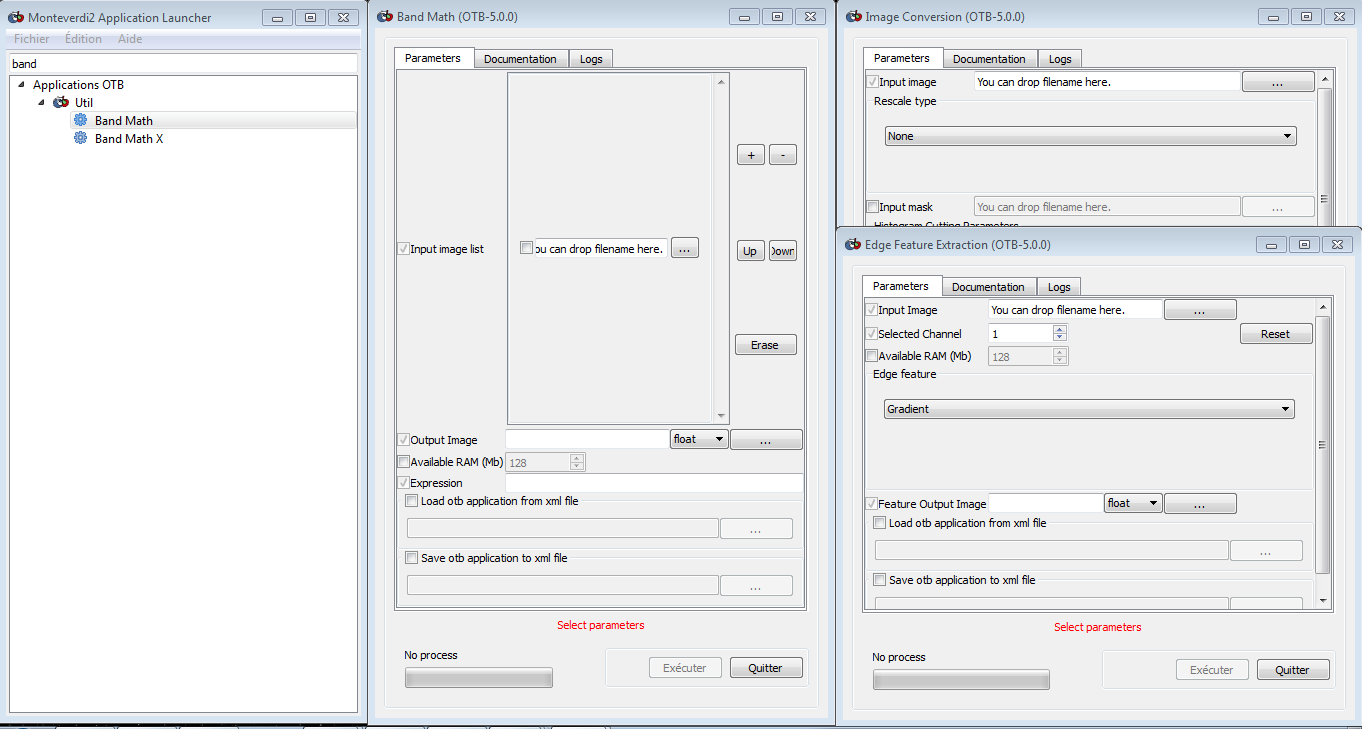
\includegraphics[scale=0.3]{images/Mapla.png} 
\end{figure}
\end{frame}

\begin{frame}
\frametitle{Monteverdi2}
Version 0.8.1: Visualization parameters persistence, layers database, OTB-Applications, french language, histogram, VW2 scene 
\begin{figure}[hbtp]
    \centering
    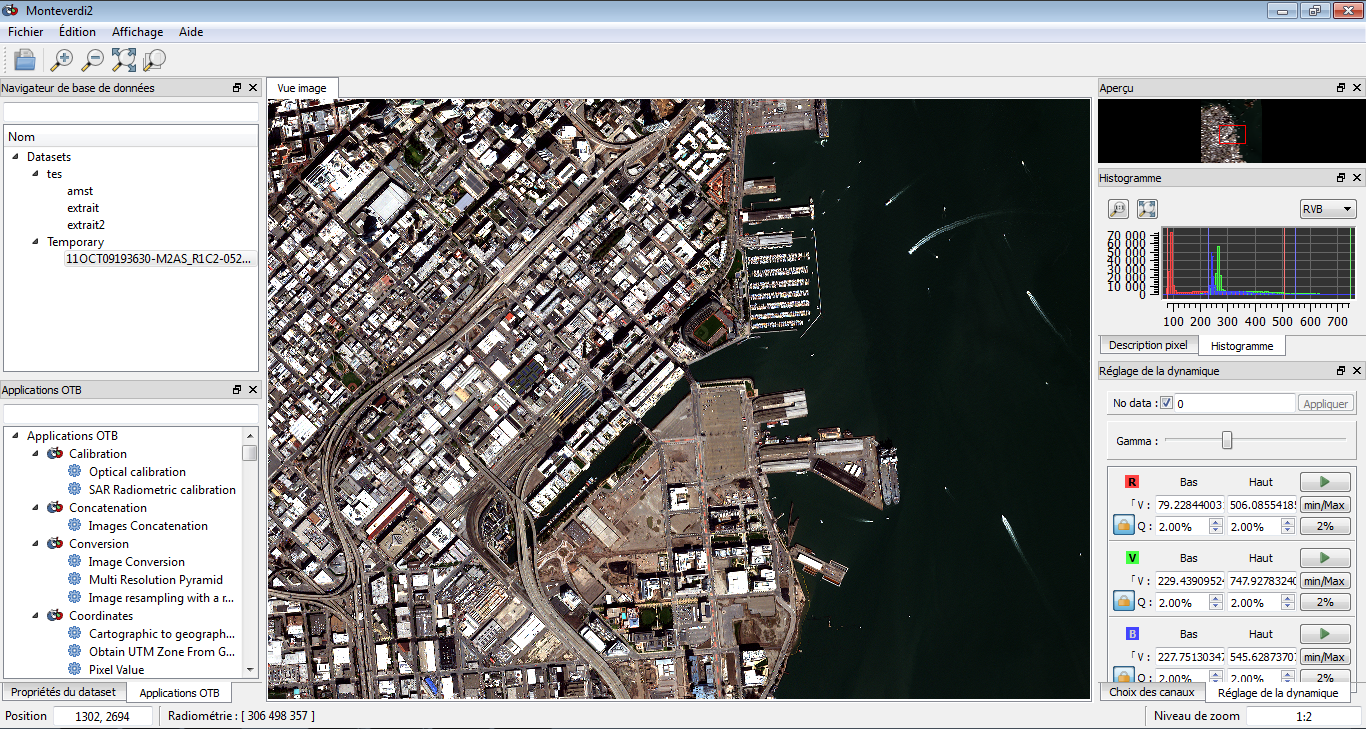
\includegraphics[scale=0.3]{images/MVD2.png} 
\end{figure}
\end{frame}

\begin{frame}
\frametitle{Mv$^{2}$}
Multi-layer view:
\begin{itemize}
 \item NEW: Multiple filename selection when using the File/Open... menu action
 \item NEW: Multiple filename input via the command-line
 \item NEW: Fast-move using the ICE rendering engine
 \item NEW: Reference layer projection combo-box chooser
 \item NEW: Zoom to extent of all layers (in addition to zoom to layer extent and zoom to 1:1 resolution)
\end{itemize}
\end{frame}


\begin{frame}
\frametitle{Mv$^{2}$}
\begin{figure}[hbtp]
    \centering
    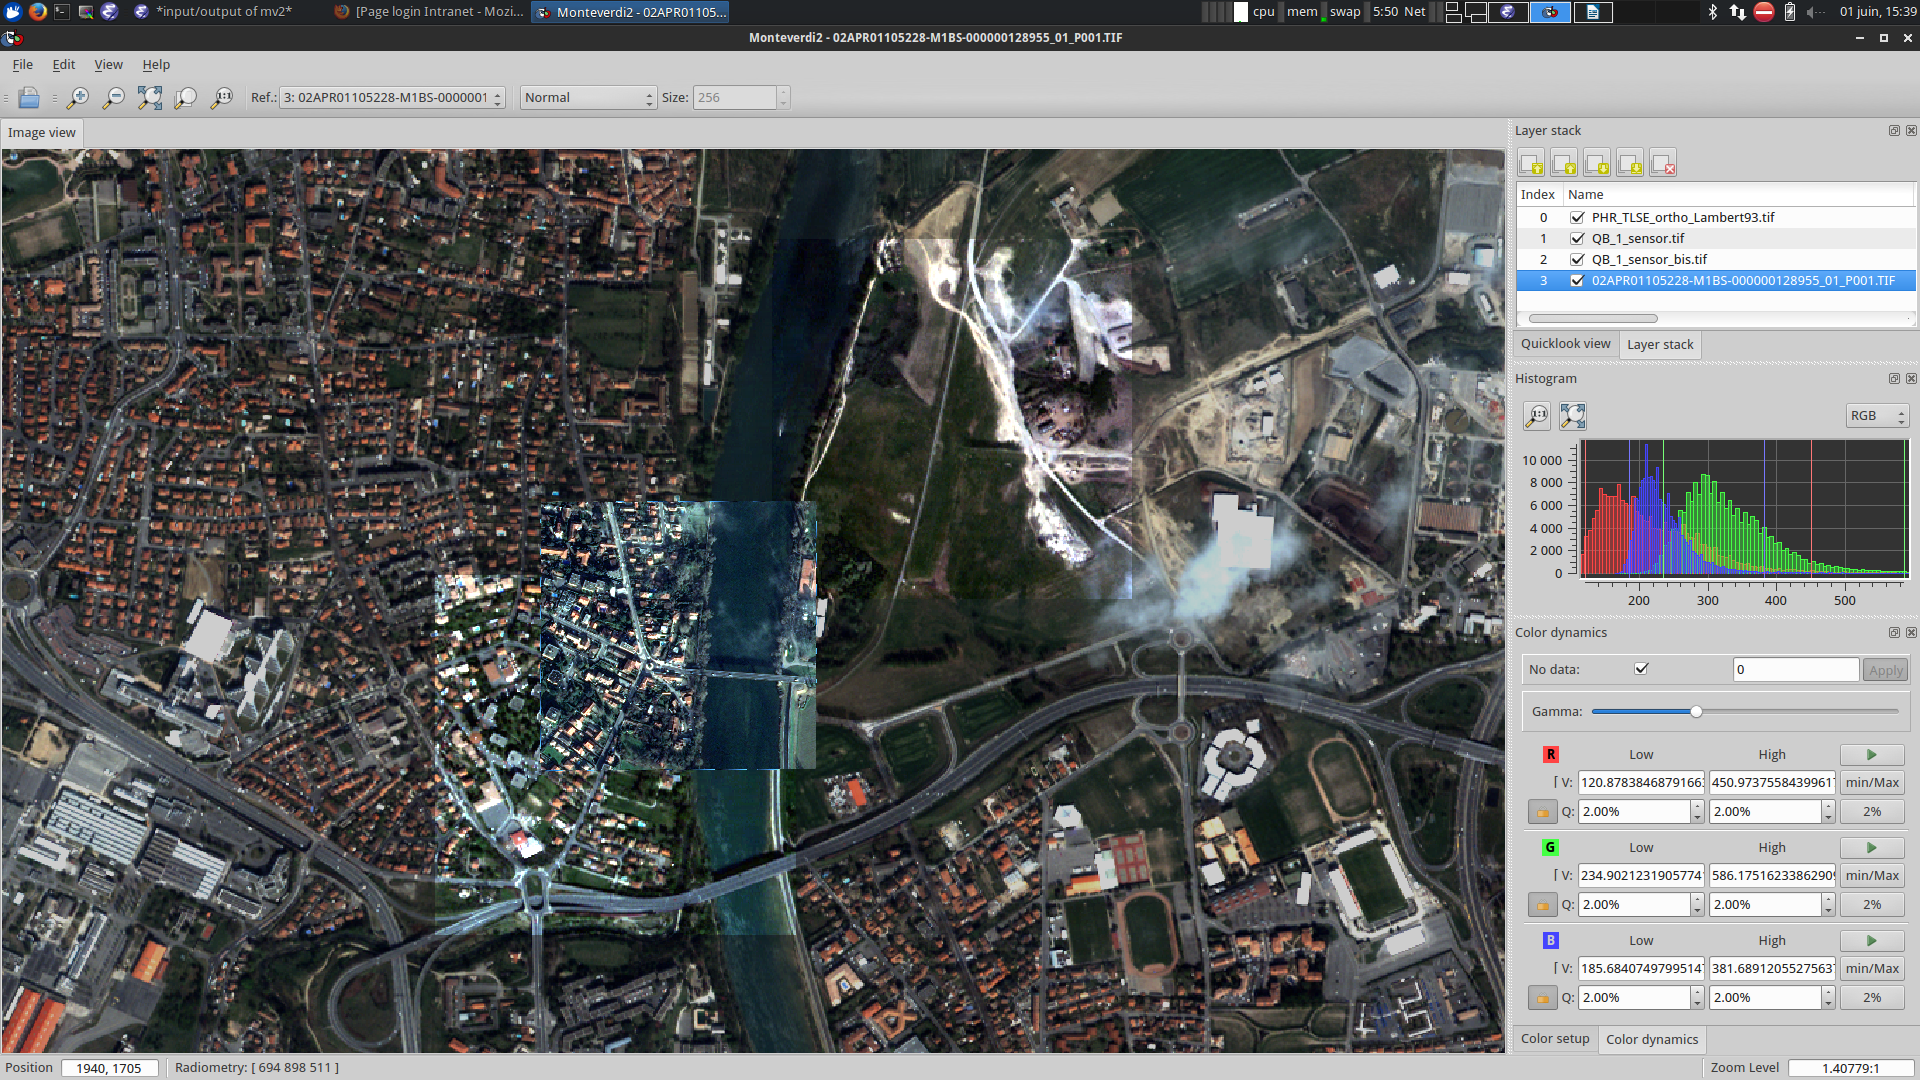
\includegraphics[scale=0.17]{images/2015-06-01_Multi-layer_1.png} 
\end{figure}
\end{frame}

\begin{frame}
\frametitle{Mv$^{2}$}
 Layer-stack and Layer-by-Layer parameters edition:
\begin{itemize}
 \item NEW: Interactive layer-stack edition (moving up/down/top/bottom, deleting)
 \item NEW: Layer-by-layer parameters edition
 \begin{itemize}
  \item Show/Hide check-bow
  \item Translucency (alpha)
  \item and all previous controls such as color-setup, color-dynamics, no-data, histogram navigation...
 \end{itemize}
\end{itemize}
\end{frame}

%% Example : translucency (alpha) slider
\begin{frame}
\frametitle{Mv$^{2}$}
\begin{figure}[hbtp]
    \centering
    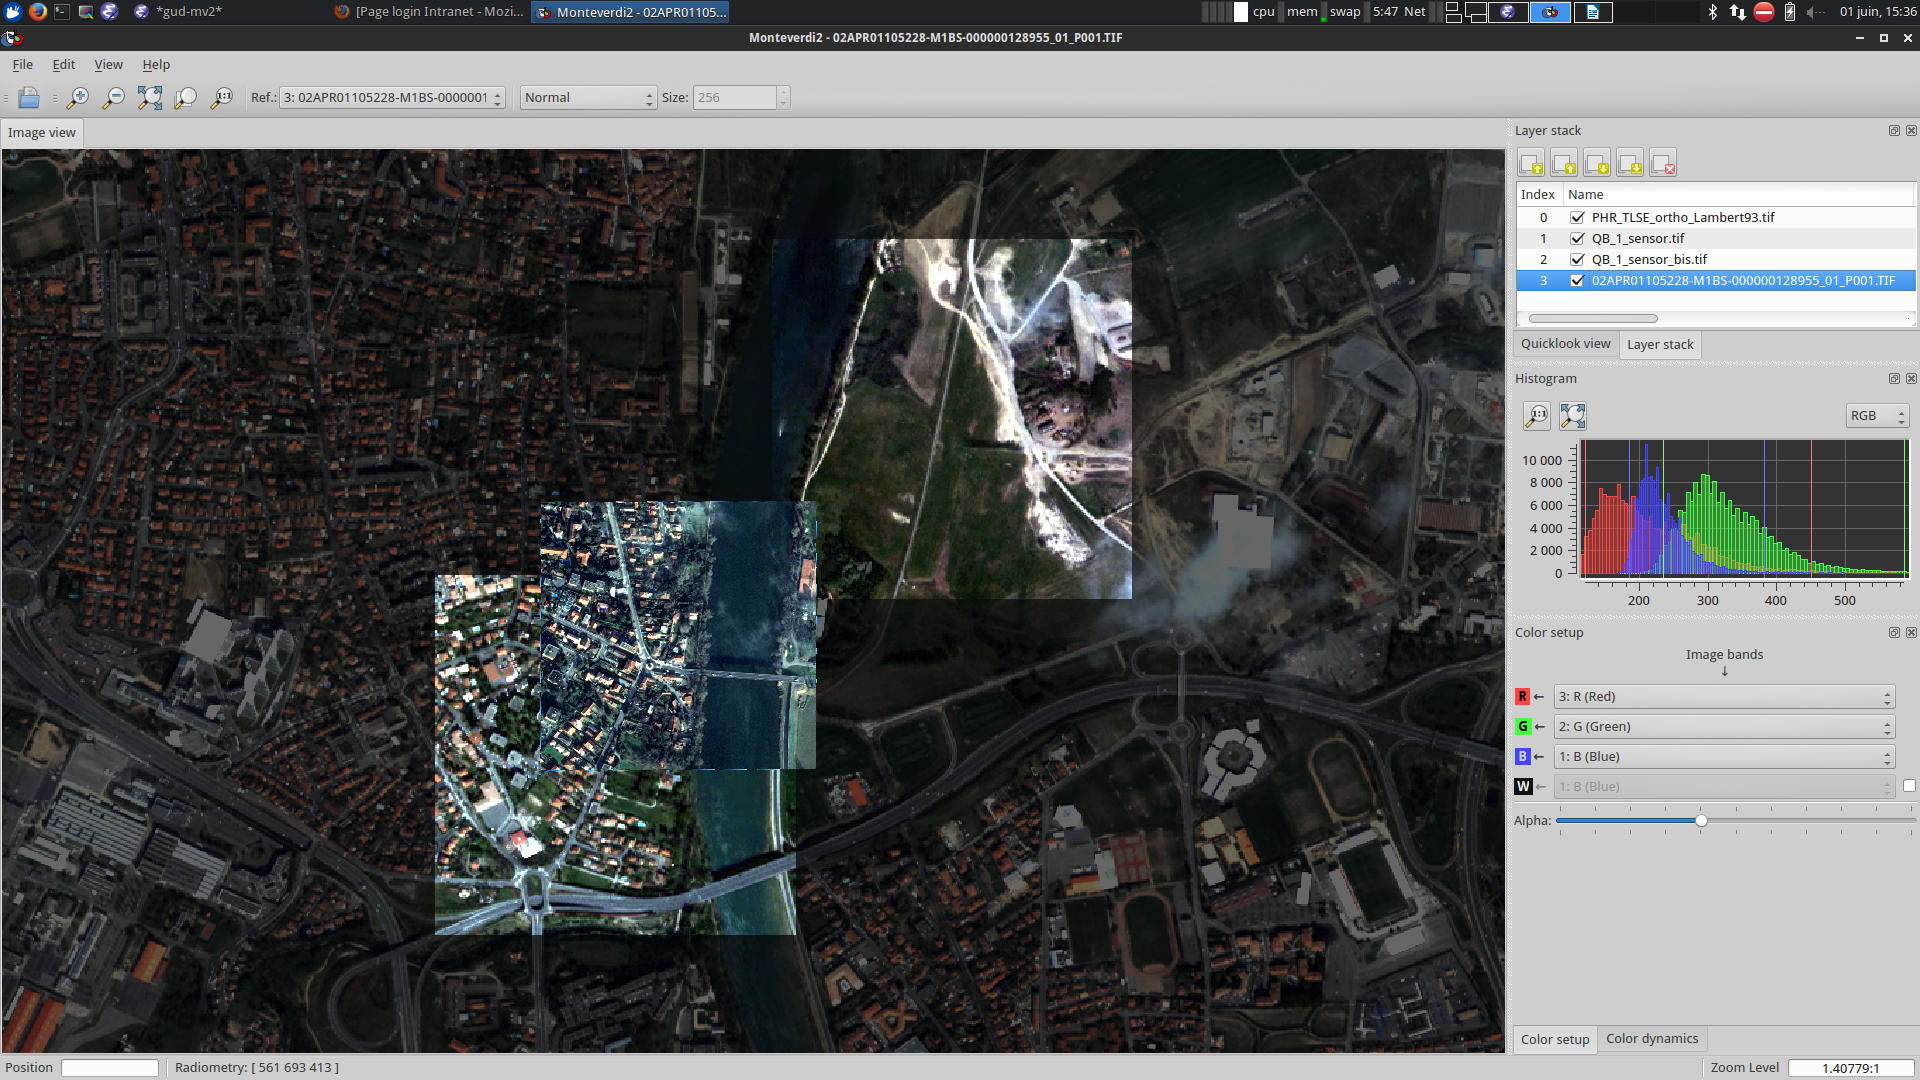
\includegraphics[scale=0.17]{images/2015-06-01_Multi-layer_2.png} 
\end{figure}
\end{frame}

\begin{frame}
\frametitle{Mv$^{2}$}
Layer-by-layer shader edition
\begin{itemize}
 \item Shader effect of the ICE rendering engine
 \begin{itemize}
    \item Chessboard
    \item Gradient
    \item Local contrast
    \item Local translucency
    \item Normal
    \item Spectral angle
    \item Swipe (horizontal/vertical)
 \end{itemize}
\end{itemize}
\end{frame}

%% Example: Local-contrast+Spectral-angle and Chessboard over translucent background

\begin{frame}
\frametitle{Mv$^{2}$}
\begin{figure}[hbtp]
    \centering
    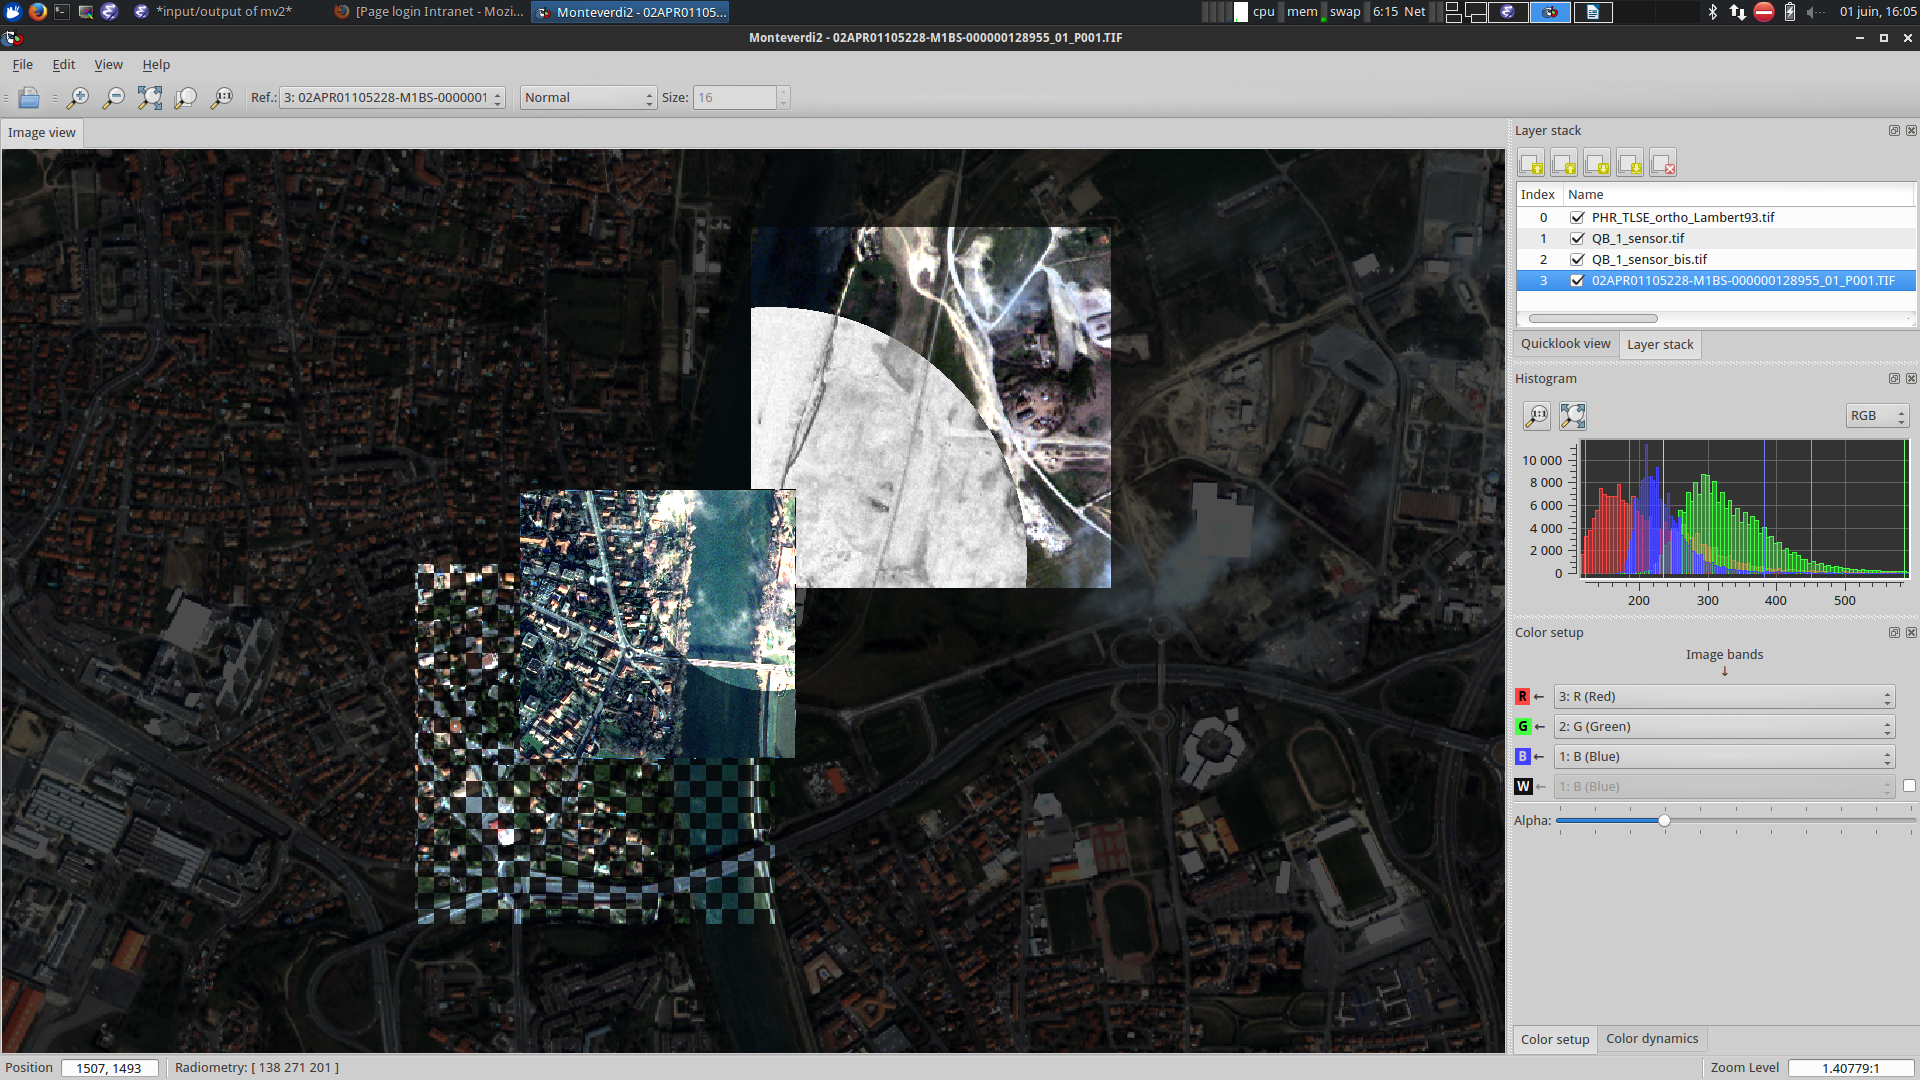
\includegraphics[scale=0.17]{images/2015-06-01_Shader-edition.png} 
\end{figure}
\end{frame}


\begin{frame}
\frametitle{Discussion for future of Monteverdi2 and its components}
Next Release of Monteverdi2 will provide the new Mv$^{2}$ features

What next?

We should select new features for the roadmap but we need new user feedback. 

Context: 
\begin{itemize}
 \item Lack of documentation blocks the user acceptance
 \item QGIS provides OTB capabilities thanks to Processing plugins 
 \item Mpnteverdi2 didn't cover all the features from Monteverdi1 (streaming processing)
\end{itemize}
\end{frame}

\end{document}
